
\let\negmedspace\undefined
\let\negthickspace\undefined
\documentclass[journal]{IEEEtran}
\usepackage[a5paper, margin=10mm, onecolumn]{geometry}
%\usepackage{lmodern} % Ensure lmodern is loaded for pdflatex
\usepackage{tfrupee} % Include tfrupee package
\setlength{\headheight}{1cm} % Set the height of the header box
\setlength{\headsep}{0mm}     % Set the distance between the header box and the top of the text
\usepackage{gvv-book}
\usepackage{gvv}
\usepackage{cite}
\usepackage{amsmath,amssymb,amsfonts,amsthm}
\usepackage{algorithmic}
\usepackage{graphicx}
\usepackage{textcomp}
\usepackage{xcolor}
\usepackage{txfonts}
\usepackage{listings}
\usepackage{enumitem}
\usepackage{mathtools}
\usepackage{gensymb}
\usepackage{comment}
\usepackage[breaklinks=true]{hyperref}
\usepackage{tkz-euclide} 
\usepackage{listings}
% \usepackage{gvv}                                        
\def\inputGnumericTable{}                                 
\usepackage[latin1]{inputenc}                                
\usepackage{color}                                            
\usepackage{array}                                            
\usepackage{longtable}                                       
\usepackage{calc}                                             
\usepackage{multirow}                                         
\usepackage{hhline}                                           
\usepackage{ifthen}                                           
\usepackage{lscape}
\renewcommand{\thefigure}{\theenumi}
\renewcommand{\thetable}{\theenumi}
\setlength{\intextsep}{10pt} % Space between text and floats
\numberwithin{equation}{enumi}
\numberwithin{figure}{enumi}
\renewcommand{\thetable}{\theenumi}
\begin{document}
\bibliographystyle{IEEEtran}
\title{12.9.4.15}
\author{EE24BTECH11041 - Mohit}
% \maketitle
% \newpage
% \bigskip
{\let\newpage\relax\maketitle}
\begin{enumerate}
\item Find the equation of a curve passing through the point \brak{0,0} and whose differential equation
 is $y^{'} = e^x\sin{x}$\\
\textbf{Theoritical Solution:-}\\

The given differential equation is:
\begin{align}
y^{'} = e^x \sin{x}
\end{align}

Integrating both sides:
\begin{align}
y &= \int e^x \sin{x}dx
\end{align}

Using integration by parts:
\begin{align}
\int e^x \sin{x}dx &= e^x \sin{x} - \int e^x \cos{x} dx
\end{align}

Let I = $\int e^x \sin{x} dx$ . Then:
\begin{align}
I &= e^x \sin{x} - \int e^x \cos{x}dx
\end{align}

Now, solve $\int e^x \cos{x}dx$ using integration by parts again:
\begin{align}
\int e^x \cos{x}dx &= e^x \cos{x} - \int e^x (-\sin{x}) dx
= e^x \cos x + \int e^x \sin{x}dx
\end{align}

Substituting back, we get:
\begin{align}
I &= e^x \sin{x} - (e^x \cos{x} + I) \\
I + I &= e^x (\sin{x} - \cos{x}) \\
2I &= e^x (\sin{x} - \cos{x}) \\
I &= \frac{e^x (\sin{x} - \cos{x})}{2}
\end{align}

Thus, the solution to the differential equation is:
\begin{align}
y &= \frac{e^x (\sin{x} - \cos{x})}{2} + C
\end{align}

Using the initial condition $ y\brak{0} = 0 $:
\begin{align}
y\brak{0} &= \frac{e^0 (\sin{0} - \cos{0})}{2} + C \\
0 &= \frac{(0 - 1)}{2} + C \\
C &= \frac{1}{2}
\end{align}

The final solution is:
\begin{align}
y &= \frac{e^x (\sin{x} - \cos{x})}{2} + \frac{1}{2}
\end{align}

\textbf{Laplace-Method}

\begin{align}
y^{'} = e^x \sin{x}
\end{align}

Taking Laplace on both sides
\begin{align}
\mathcal{L}\brak{y^{'}} = \mathcal{L}\brak{e^x \sin{x}}
\end{align}
Let,
\begin{align}
\mathcal{L}\brak{y^{'}} = sY\brak{s} \text{ and } \mathcal{L}\brak{e^x \sin{x}} = G\brak{s}
\end{align}
Subsituting in 1.16,
\begin{align}
sY\brak{s} = G\brak{s}\\
\frac{Y\brak{s}}{G\brak{s}}=\frac{1}{s}
\end{align}
Applying bi-linear Transformation
\begin{align}
s = \frac{2}{h}\brak{\frac{1+z^{-1}}{1-z^{-1}}}\\
\end{align}
Subsituting in 1.19,
\begin{align}
\frac{Y\brak{s}}{G\brak{s}}=\frac{h}{2}\brak{\frac{1+z^{-1}}{1-z^{-1}}}\\
\brak{1-z^{-1}}Y\brak{s}=\frac{h}{2}\brak{1+z^{-1}}G\brak{s}\\
Y\brak{s} - z^{-1}Y\brak{s} = \frac{h}{2}\brak{G\brak{s}-z^{-1}G{s}}
\end{align}
Then putting the value of $Y\brak{s}$ and $G\brak{s}$\\
Final expression :-
\begin{align}
y_n - y_{n-1} = \frac{h}{2}\brak{e^x_n \sin{x_n} + e^{x-1}_n \sin{x_{n-1}}}
\end{align}

\textbf{Trapezoid Rule :-}\\

The trapezoidal rule is as follows.
\begin{align}
    A &= \int_a^b f\brak{x}\, dx \approx h\brak{\frac{1}{2}f\brak{a} + f\brak{x_1} + f\brak{x_2} \cdots + f\brak{x_{n-1}} + \frac{1}{2}f\brak{b}}\\
    h &= \frac{b-a}{n}\\
    A &= j_n, \text{ where, } j_{i + 1} = j_i + h\frac{f\brak{x_{i+1}} + f\brak{x_i}}{2}\\ 
        \xrightarrow{} j_{i + 1} &= j_i + h\brak{\sqrt{x_{i+1}}+\sqrt{x_{i}}}\\
    x_{i+1} &= x_i + h\\
\end{align}
\begin{figure}[h!]
   \centering
   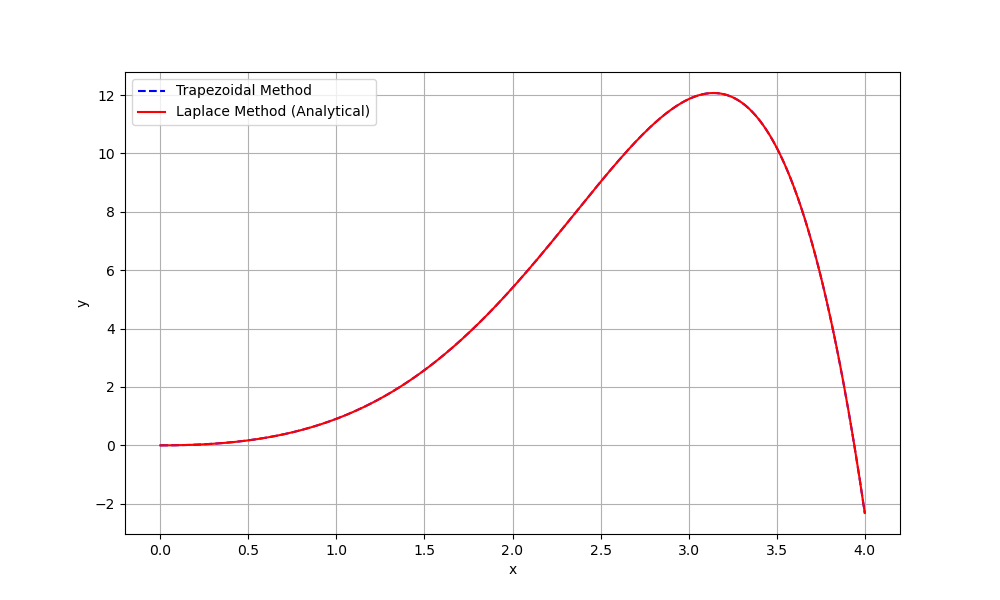
\includegraphics[width=0.7\linewidth]{figs/Figure_1.png}
\end{figure}   
 

\end{enumerate}
\end{document}
